\documentclass{article}

\usepackage[pdf]{graphviz}
\usepackage{ragged2e}
\usepackage[pdftex]{graphicx}
\usepackage[utf8]{inputenc}			% кодировка исходного текста
\usepackage[english,russian]{babel}	% локализация и переносы
\usepackage{lscape}
\usepackage{listings}
% Математика
\usepackage{morewrites}
\usepackage{amsmath,amsfonts,amssymb,amsthm,mathtools,amstext} 
\usepackage{amsmath}
\usepackage{geometry}

\begin{document}

\section{Машины Тьюринга}

Работу требуется выполнять в системе \url{turingmachine.io}. \\\\
Для сдачи заданий 1-2 требуется прикрепить файлы YAML с исходным кодом проекта. Каждый файлы должен иметь наименование задание\_пункт.yml, к примеру 1\_1.yml для первой задачи первого задания. \\\\

\subsection{Операции с числами}

Реализуйте машины Тьюринга, которые позволяют выполнять следующие операции:
\begin{enumerate}
    \item Сложение двух унарных чисел (1 балл) \\
        Алгоритм:
        \begin{enumerate}
            \item Движемся вправо по 1, пока не достигнем +
            \item Когда достигли +, заменяем его на 1 и смещаемся влево
            \item Движемся влево по 1, пока не достигнем $\lambda$, после того как достигли, смещаемся вправо
            \item Первую встретившуюся 1 заменяем на $\lambda$ и смещаемся вправо
            \begin{lstlisting}
                input: '111+11'
                blank: ' '
                start state: start
                table:
                start:
                    [1]: R
                    +  : {write: 1, L: del}
                del:
                    [1]: L
                    ' ': {write: ' ', R: step}
    
                step:
                    1 : {write: ' ', R: done}
  
                done:
            \end{lstlisting}
        \end{enumerate}
    
    \item Умножение унарных чисел (1 балл) \\
        Алгоритм:
        \begin{enumerate}
            \item Ищем второй множитель, заменяем в нём первую 1 на x
            \item Если встретили $\lambda$, то ставим =
            \item Идём от знака = до первого множителя и замеянем все 1 на х
            \item После того, как в первом множителе не осталось 1, возвращаем их на место и также ставим ещё один x во втором множителе
            \item Повторяем эту операцию, пока во втором множителе не будет столько х, сколько там было 1 изначально, как только набралось такое количество, заменяем x на 0.
            
            \begin{lstlisting}
            # Adds 1 to a binary number.
            input: '111*11'
            blank: ' '
            start state: v1
            table:
            v1:
                1: R
                '*' : {R: v2}
    
            v2:
                1: {write: 'x', R: v3}
                '=': {L: v11}
                x: R
  
            v3:
                1: R
                ' ': {write: '=', L: v4}
                '=': {L: v4}
    
            v4:
                1: {L: v5}
                x: {L: v5}
    
            v5: 
                1: L
                x: L
                '*' : {L: v6}
    
            v6: 
                x: L
                1: {write: 'x', R: v8}
                ' ' : {R: v7}
  
            v7: 
                x: {write: '1', R: v7}
                '*': {R: v2}
  
            v8:
                '*': R
                1: R
                x: R
                '=': {R: v9}
  
            v9:
                1: R
                ' ': {write: '1', L: v10}
    
            v10:
                1: L
                '=': {L: v4}
    
            v11:
                x: {write: '1', L: v11}
                '*': {L: v12}
    
            v12:

            \end{lstlisting}
        \end{enumerate}
\end{enumerate}


\subsection{Операции с языками и символами}

Реализуйте машины Тьюринга, которые позволяют выполнять следующие операции:
\begin{enumerate}
    \item Принадлежность к языку $L = \{ 0^n1^n2^n \}, n \ge 0$ (0.5 балла)
    \begin{enumerate}
        \item Поочерёдно заменяем 0,1 и 2 на временный символ a, затем возвращаемся назад в начало слова и повторяем процесс
        \item Если при выполнении первого шага с распознаванием нуля мы находим пустой символ, то переходим к состоянию успеха: удаляем строку и печатаем символ s
        \item Если посреди последовательности из 0, 1 или 2 мы находим другой символ, то переходим в 
        состояние неуспеха: удаляем всю строку и печатаем символ f
        \begin{lstlisting}
            input: '0011222'
            blank: ' '
            start state: v0
            table:

            v0:
                ' ': {L: v4}
                0: {write: a, R: v1}
                [1, 2]: {R: v5}
                a: R

            v1:
                [0, a]: R
                1: {write: a, R: v2}
                [2, ' ']: {L: v5}

            v2:
                [1, a]: R
                2: {write: a, L: v3}
                [0,' ']: {L: v5}

            v3:
                [a, 2, 1, 0]: L
                ' ': {R: v0}

            v4:
                a: {write: ' ', L}
                ' ': {write: s, R: v7}

            v5:
                [a, 0, 1, 2]: R
                ' ': {L: v6}

            v6:
                [a, 0, 1, 2]: {write: ' ', L}
                ' ': {write: f, R: v7}
            v7:
                ' ': L
        \end{lstlisting}
    \end{enumerate}
    \item Проверка соблюдения правильности скобок в строке (минимум 3 вида скобок) (0.5 балла)
    \begin{enumerate}
        \item Находим первую правую скобку
        \item Затем проверяем предшествующую ей, если на такого же типа, то заменяем обе на временный символ a и переходим в начальное состояние, иначе переходим в состояние неуспеха: удаляем строку и печатаем f.
        \item Если переходя обратно в начальное состояние мы находим конец строки, то переходим в состояние успеха: печатаем символ s и удаляем остальную строку.
        \begin{lstlisting}
            input: '([({})])({[]}){}'
            blank: ' '
            start state: v1
            table:
            v1:
                ' ': {L: v8}
                a: R
                ['(','[','{']: {R: v2}
                ')': {write: a, L: v3}
                ']': {write: a, L: v4}
                '}': {write: a, L: v5}

            v2:
                ' ': {L: v12}
                 a: R
                ['(','[','{']: R
                ')': {write: a, L: v3}
                ']': {write: a, L: v4}
                '}': {write: a, L: v5}

            v3:
                a: L
                '(': {write: a, L: v6}
                 ['{', '[']: {write: a, L: v12}
                ' ': {R: v12}

            v4:
                 a: L
                '[': {write: a, L: v6}
                ['{', '(']: {write: a, L: v12}
                ' ': {R: v12}

            v5:
                a: L
                '{': {write: a, L: v6}
                ['(', '[']: {write: a, L: v12}
                ' ': {R: v12}

            v6:
                ' ': {R: v1}
                [a, '{', '[', '(']: {R: v7}

            v7:
                a: {L: v1}
                ' ': L

            v8:
                ' ': {R: v9}
                a: L
                ['{', '[', '(']: {L: v6}

            v9:
                [a, ' ']: {write: d, R: v10}

            v10:
                [a, '{', '[', '(', '}', ']', ')']: R
                ' ': {L: v11}

            v11: 
                [a, '{', '[', '(', '}', ']', ')']: {write: ' ', L}
                d: L
                ' ': {R: v13}

            v12:
                [a, '{', '[', '(', '}', ']', ')', ' ']: {R: v10}

            v13:
                ' ': {write: f, R: v7}
        \end{lstlisting}
    \end{enumerate} 
    
    \item Поиск минимального по длине слова в строке (слова состоят из символов 1 и 0 и разделены пробелом) (1 балл)
    \begin{enumerate}
        \item Если первое слово длиннее, стираем его и восстанавливаем его из временных символов
        \item Если второе слово оказалось больше, копируем первое на место второго и удаляем то, что осталось от второго
        \begin{lstlisting}
            input: '1010 010 01 000'
            blank: ' '
            start state: v1
            table:
            v1:
                0: {write: a, R: v2}
                1: {write: b, R: v2}
                [a, b]: R
                ' ': {L: v9}
            v2:
                [0, 1]: R
                ' ': {R: v3}
            v3:
                 ' ': {L: v7}
                 0: {write: a, L: v5}
                 1: {write: b, L: v5}
                 [a, b]: {R: v4}
            v4:
                [a, b]: R
                0: {write: a, L: v5}
                1: {write: b, L: v5}
                ' ': {L: v22}
            v5:
                [a, b]: L
                ' ': {L: v6}
            v6:
                [0, 1, a, b]: L
                ' ': {R: v1}
            v7:
                ' ': {L: v8}
            v8:
                a: {write: 0, L}
                b: {write: 1, L}
                [0, 1]: L
                ' ': {R: done}
            v9:
                [a, b]: L
                ' ': {R: v10}
            v10:
                a: {write: 0, R}
                b: {write: 1, R}
                ' ': {R: v11}
            v11:
                [a, b, 0, 1]: {write: a, R}
                ' ': {L: v12}
            v12:
                a: L
                ' ': {L: v13}
            v13:
                [a, b]: L
                0: {write: a, R: v14}
                1: {write: b, R: v17}
                ' ': {R: v20}
            v14:
                [a, b]: R
                ' ': {R: v15}
            v15:
                a: R
                [0, 1, ' ']: {L: v16}
            v16:
                a: {write: 0, L: v12}
                ' ': {L: v12}
            v17:
                [a, b]: R
                ' ': {R: v18}
            v18:
                a: R
                [0, 1, ' ']: {L: v19}
            v19:
                a: {write: 1, L: v12}
                ' ': {L: v12}
            v20:
                [a, b]: {write: ' ', R}
                [0, 1]: {L: v6}
                ' ': {R: v21}
            v21:
                [a, b]: {write: ' ', R}
                [0, 1]: {L: v6}
                ' ': {R: done}
            v22:
                [a, b]: L
                ' ': {L: v23}
            v23:
                [0, 1, a, b]: L
                ' ': {R: v24}
            v24:
                [0, 1, a, b]: {write: ' ', R}
                ' ': {R: v25}
            v25:
                a: {write: 0, R}
                b: {write: 1, R}
                ' ': {L: v6}
            done:
        \end{lstlisting}
    \end{enumerate}
    
    
\end{enumerate}


\section{Квантовые вычисления}

Для выполнения заданий по квантовым вычислениям требуется QDK. Его можно скачать здесь: \url{https://docs.microsoft.com/en-us/azure/quantum/install-overview-qdk}. 
\\\\
Но можно использовать любой пакет, типа \url{https://qiskit.org/}. 
\\\\
В качестве решения задачи надо предоставить схему алгоритма для частного случая при фиксированном количестве кубитов и фиксированных состояниях. 


\subsection{Генерация суперпозиций 1 (1 балл)}

Дано $N$ кубитов ($1 \le N \le 8$) в нулевом состоянии $\Ket{0\dots0}$. Также дана некоторая последовательность битов, которое задаёт ненулевое базисное состояние размера $N$. Задача получить суперпозицию нулевого состояния и заданного.

$$\Ket{S} = \frac{1}{\sqrt2}(\Ket{0\dots0} +\Ket{\psi})$$

То есть требуется реализовать операцию, которая принимает на вход:

\begin{enumerate}
    \item Массив кубитов $q_s$
    \item Массив битов $bits$ описывающих некоторое состояние $\Ket{\psi}$. Это массив имеет тот же самый размер, что и $qs$. Первый элемент этого массива равен $1$.
\end{enumerate}

\begin{enumerate}
    \item В начале у нас есть N независимых кубитов |0>
    \item Первые кубиты векторов различны, применим оператор Адамара к первому кубиту
    \item Все кубиты qs = 0, если кубит bits[i] = 1, то нужно запутать i-ый кубит, а если bits[i] = 0, то не нужны, т.к. кубиты совпадают и равны 0
\end{enumerate}

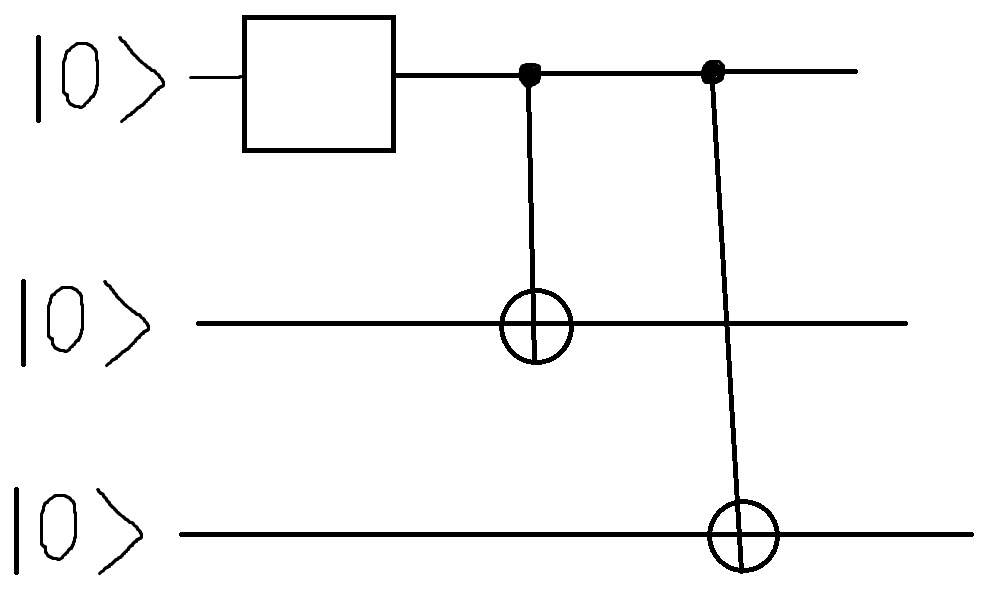
\includegraphics[scale=0.5]{1.jpg}

Заготовка для кода:
\begin{lstlisting}
	namespace Solution
	 {
	    open Microsoft.Quantum.Primitive;
	    open Microsoft.Quantum.Canon;
	    
	    operation Solve(qs: Qubit[], bits: Bool[]) : () 
	    {
	        body 
	        { 
	            H(qs[0]);
	            for (i in 1..Length(qs) - 1)
	             {
	                if (bits[i])
	                 {
	                    CNOT(qs[0], qs[i]); 
	                } 
	            }                  
	        }
	    }
	}
\end{lstlisting}


\subsection{Различение состояний 1 (1 балл)}

Дано $N$ кубитов ($1 \le N \le 8$), которые могут быть в одном из двух состояний:

$$\Ket{GHZ} = \frac{1}{\sqrt2}(\Ket{0\dots0} +\Ket{1\dots1})$$
$$\Ket{W} = \frac{1}{\sqrt N}(\Ket{10\dots00}+\Ket{01\dots00} + \dots +\Ket{00\dots01})$$

Требуется выполнить необходимые преобразования, чтобы точно различить эти два состояния. Возвращать $0$, если первое состояние и 1, если второе. 
\begin{enumerate}
    \item Чтобы измерить состояние системы надо измерить кубиты
    \item При N > 1 состояние 1: N нулей, либо N единиц, состояние 2: 1 единица
    \item При N = 1 состояния не различать (в обоих состояниях может выпасть вектор, который содержит 1 единицу)
\end{enumerate}
Заготовка для кода:
    \begin{lstlisting}
        namespace Solution {
            open Microsoft.Quantum.Primitive;
            open Microsoft.Quantum.Canon;
            operation Solve (qs : Qubit[]) : Int 
            {
                body
                {
                    mutable ones = 0;
                    for i in 0..Length(qs) - 1 {
                        if (M(qs[i]) == One) {  // measurement
                            set ones += 1;
                        }
                    }
                    if (ones == 1) {
                        return 1;
                    }
                    return 0;
                }
            }
        }
    \end{lstlisting}


\subsection{Различение состояний 2 (2 балла)}

Дано $2$ кубита, которые могут быть в одном из двух состояний:

$$\Ket{S_0} = \frac{1}{2}(\Ket{00} + \Ket{01} + \Ket{10} + \Ket{11})$$
$$\Ket{S_1} = \frac{1}{2}(\Ket{00} - \Ket{01} + \Ket{10} - \Ket{11})$$
$$\Ket{S_2} = \frac{1}{2}(\Ket{00} + \Ket{01} - \Ket{10} - \Ket{11})$$
$$\Ket{S_3} = \frac{1}{2}(\Ket{00} - \Ket{01} - \Ket{10} + \Ket{11})$$


Требуется выполнить необходимые преобразования, чтобы точно различить эти четыре состояния. Возвращать требуется индекс состояния (от $0$ до $3$). 
\\\\
Заготовка для кода:
\begin{lstlisting}
namespace Solution {
        open Microsoft.Quantum.Primitive;
        open Microsoft.Quantum.Canon;
        operation Solve (qs : Qubit[]) : Int
        {
            body
            {

                return 
            }
        }
}
\end{lstlisting}


\subsection{Написание оракула 1 (2 балла)}

Требуется реализовать квантовый оракул на $N$ кубитах ($1 \le N \le 8$), который реализует следующую функцию: $f(\pmb{x}) = (\pmb{b}\pmb{x}) \mod 2$, где  $\pmb{b} \in \{0,1\}^N$ вектор битов и  $\pmb{x}$ вектор кубитов. Выход функции записать в кубит $\pmb{y}$. Количество кубитов $N$ ($1 \le N \le 8$). 
\\\\
Заготовка для кода:
\begin{lstlisting}
namespace Solution {
        open Microsoft.Quantum.Primitive;
        open Microsoft.Quantum.Canon;
        operation Solve (x : Qubit[], y : Qubit, b : Int[]) : ()
        {
            body
            {

            }
        }
}
\end{lstlisting}

\end{document}